\section[Neurosymbolic Architecture for Novelty Handling]{A Neurosymbolic Architecture for Open-World Novelty Handling}
\label{sec:architecture}

RAPid-Learn addresses the specific problem of recovering from execution impasses caused by novelty. However, a complete open-world agent must handle the full lifecycle of novelty: detecting that something has changed, characterizing the nature of the change, exploring the environment to gather information, and accommodating the novelty to continue task performance. This section presents a neurosymbolic cognitive architecture~\citep{goel2024neurosymbolic} that integrates RAPid-Learn within a broader framework for novelty handling. The architecture combines symbolic inference, neural inference, and reinforcement learning, with each component contributing to different aspects of novelty detection and accommodation.

The architecture provides a concrete instantiation of the claim developed in \cref{sec:abstractions}: that structured abstractions over actions determine whether novelty-induced mismatch can be resolved efficiently. The operator--executor decomposition is the structural feature that enables the cascading recovery pipeline described below---without it, execution failures would propagate as undifferentiated performance degradation, and the architecture would have no principled basis for selecting among recovery strategies.

\subsection{Novelty Typology for Goal-Oriented Agents}
\label{sec:novelty_typology}

The architecture's recovery strategies are organized around the four-way novelty taxonomy developed in \cref{sec:novelty_taxonomy}: prohibitive, obstructive, beneficial, and nuisance novelties. For a goal-oriented agent equipped with a symbolic planner, the functional impact of a novelty depends on how it affects the agent's ability to generate and execute plans~\citep{goel2024neurosymbolic}. The taxonomy maps to recovery strategies as follows.

Prohibitive novelties (\cref{def:prohibitive}) prevent the agent from generating any valid plan---for example, if the crafting table is removed from the environment. These trigger plan-level exploration, in which the agent searches for new knowledge (entities, operators, or recipes) that would restore plannability. Obstructive novelties (\cref{def:obstructive}) are the primary focus of RAPid-Learn: the agent has a valid plan, but execution fails at a specific operator. The axe novelty from the running example is obstructive---the \texttt{break} operator's executor fails because trees are now unbreakable without an axe. These invoke the failure recovery pipeline described in \cref{sec:failure_recovery}, culminating in the RAPid-Learn executor learner if symbolic strategies are insufficient. Beneficial novelties (\cref{def:beneficial}) are exploited when discovered, and nuisance novelties (\cref{def:nuisance}) are identified and ignored.

The distinction between prohibitive and obstructive novelties is operationally significant because they require different recovery strategies: prohibitive novelties demand symbolic model revision (new operators or fluents), while obstructive novelties demand new executors for existing operators. This distinction is finer-grained than the three-way classification used in the NovelGridworlds benchmark (\cref{sec:ngw_novelty_taxonomy}), where the \emph{detrimental} category encompasses both prohibitive and obstructive novelties.


\subsection{Architecture Overview}
\label{sec:arch_overview}

The architecture, depicted in \cref{fig:architecture}, consists of four main components that interact through the agent's knowledge repository $\mathcal{K} = (\KB, \Theta)$, where $\KB$ stores symbolic knowledge (facts, rules, operators in first-order logic) and $\Theta$ stores subsymbolic knowledge (neural network parameters). The components are:

\begin{figure}[htbp]
    \centering
    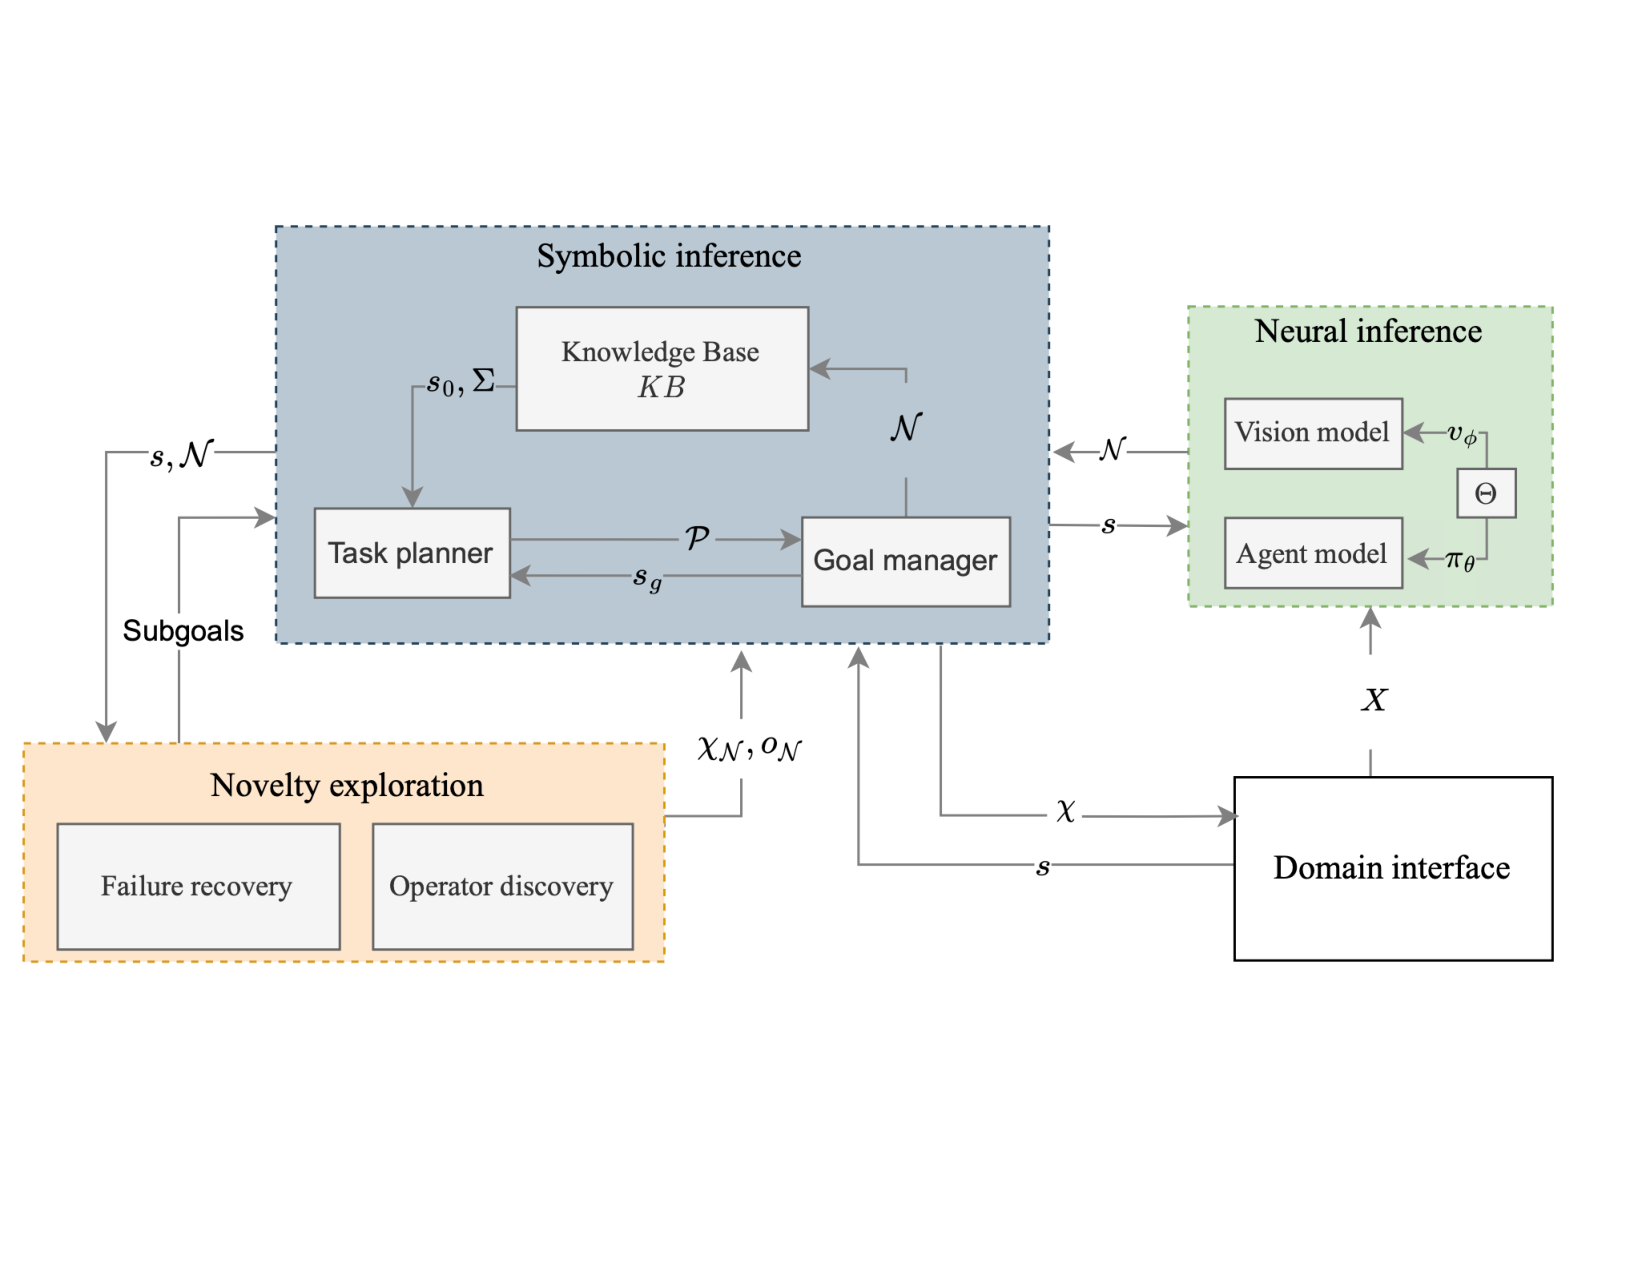
\includegraphics[width=\textwidth]{figures/chapter5/diarcgram.pdf}
    \caption[Neurosymbolic architecture for novelty handling]{High-level architecture of the neurosymbolic cognitive architecture for novelty handling. The four main components communicate through the shared knowledge repository $\mathcal{K} = (\KB, \Theta)$. Symbolic inference (task planner, goal manager) generates and executes plans, detecting novelties through expectation violations. Neural inference (vision model, agent model) detects visual and behavioral anomalies and asserts novelty descriptions into $\KB$. When execution fails, the novelty exploration component applies a cascading sequence of recovery strategies---culminating in the RAPid-Learn executor learner---interacting with the environment through the domain interface, which mediates symbolic state observations, images, and LiDAR sensor data.}
    \label{fig:architecture}
\end{figure}

\paragraph{Symbolic inference.} The knowledge base $\KB$ stores facts about the environment using a first-order language, including entity properties, spatial relations, and the planning domain (operators with preconditions and effects, specified in PDDL). The \emph{task planner} retrieves the domain definition and current state from $\KB$ and searches for a plan. The \emph{goal manager} orchestrates plan execution: it verifies operator preconditions against the observed state, dispatches executors through the domain interface, monitors whether effects match expectations, and detects novelties when predictions diverge from observations. The general principle for symbolic novelty detection is predicting the next state and comparing the prediction with the observed state---any discrepancy constitutes a potential novelty.

\paragraph{Neural inference.} Two neural components supplement symbolic novelty detection. A \emph{vision model}, based on a deep autoencoder~\citep{abati2019autoregression}, detects visual novelties by monitoring reconstruction error on image observations---novel visual elements produce higher reconstruction error than familiar ones. An \emph{agent model}, trained via behavioral cloning on trajectories of known actor types, monitors other actors' behavior and detects when their actions are unlikely under the learned behavioral model. Both components produce symbolic novelty descriptions that are asserted into $\KB$ for further reasoning.

\paragraph{Novelty exploration.} When novelty is detected, the \emph{novelty exploration} component employs a cascading sequence of recovery strategies, progressing from lightweight symbolic approaches to more expensive learning-based methods. The strategies are organized around the type of failure encountered, as described in \cref{sec:novelty_exploration}.

\paragraph{Domain interface.} The domain interface mediates all interactions between the agent and the environment, translating between the agent's internal representations and the environment's state and action formats. It provides both symbolic state descriptions (for the planner and goal manager) and subsymbolic observations such as images (for the vision model) and LiDAR-like sensor data (for executors).


\subsection{Symbolic Inference}
\label{sec:symbolic_inference}

\rev{Symbolic inference is performed by the \emph{goal manager} and \emph{task planner} operating on the facts and rules stored in $\KB$, both to solve the task $\PlanningTask$ and to detect novelties $\Novelty$.}

\rev{\paragraph{Knowledge base.} The knowledge base $\KB$ stores facts about symbolic state descriptions $\SymStates$ using the first-order language $\Language$. It is populated with facts and rules defined \emph{a priori} and refined through interaction with the environment, including objects, actors, functions, symbolic state representations, and a semantic type hierarchy used to describe planning tasks. During execution, other components may assert, retract, or query facts in $\KB$ to detect novelty, create plans, or store new knowledge. Because $\KB$ is the symbolic component of the knowledge repository against which novelties are defined, once information about a detected and explored novelty is asserted into $\KB$, subsequent encounters with it are no longer novel. This holds even for novelties detected through neural inference, as those are eventually expressed in $\Language$ and stored in $\KB$.}

\rev{\paragraph{Task planner.} The task planner receives a desired goal state description $\Goal$ from the goal manager, retrieves a planning domain definition $\PlanningDomain$ (operators, predicates, functions) and an initial state description $\SymState_0$ from $\KB$ to form a planning task $\PlanningTask$, and searches for a plan $\Plan$ that solves it. Whether or not a plan is found---along with the plan itself---is returned to the goal manager for further inference and execution. The planner is agnostic to the specific search algorithm; the implementation uses the off-the-shelf MetricFF planner~\citep{hoffmann2003metricff}.}

\rev{\paragraph{Goal manager.} The goal manager maintains the agent's top-level goal(s) and detects novelties in symbolic state descriptions. It submits goals to the task planner and performs inference on state descriptions, a process during which novelties of different types may surface due to planning failure, execution failure, or unexpected aspects of state descriptions. The general principle for detecting novelty with symbolic inference is to predict the next environment state and compare the prediction with the observed state; any discrepancy is a candidate novelty. Once a novelty is detected, the goal manager produces a symbolic description of it---containing the environment state, the aspects that are novel, and any operators exhibiting unexpected behavior---and asserts it to $\KB$. The different novelty types manifest through distinct symbolic signals:}

\begin{itemize}[leftmargin=*]
    \item \rev{\emph{Prohibitive novelties} are most often encountered as a failure of the task planner: if the planner cannot find a plan for a goal that is assumed achievable, the failure may signal a prohibitive novelty.}
    \item \rev{\emph{Obstructive novelties} are most often encountered as plan execution failures. During execution the goal manager verifies each operator's preconditions $\Pre_\Operator$ against the observed state; if preconditions that should hold do not, this constitutes a novelty. If preconditions hold, the executor is dispatched, and the goal manager checks whether the operator's effects $\Eff_\Operator$ are realized. An executor that fails when success was anticipated, or that succeeds but produces effects inconsistent with expectations, constitutes an obstructive novelty.}
    \item \rev{\emph{Beneficial and nuisance novelties} may arise even when the task succeeds: whenever the inferred state does not match the observed state, a novelty is registered regardless of its impact on the task.}
\end{itemize}

\rev{In all cases where novelty is detected, a symbolic description is asserted to $\KB$ and passed to the novelty exploration component, which selects an exploration policy based on how the novelty was encountered.}


\subsection{Neural Inference}
\label{sec:neural_inference}

\rev{The neural inference components detect novelty in the subsymbolic observations $X$ (e.g.,\ images) and in statistical regularities among elements of the symbolic state descriptions. Their parameters are stored in the subsymbolic knowledge repository $\Theta$. Because these components are supporting machinery rather than the core contribution of this chapter, we summarize them only briefly; full detail appears in~\citet{goel2024neurosymbolic}. A general design principle for both is caution: conservative detection thresholds are used to minimize false positives, since spurious detections trigger superfluous exploration that can hinder task performance.}

\rev{\paragraph{Vision model.} The vision model detects visual novelty from a color image of the agent's current view. It follows a deep autoencoder approach~\citep{abati2019autoregression}: an encoder maps an image to a code vector and a decoder reconstructs it, and the reconstruction error $r(\tilde{X}) = \lVert \tilde{X} - d_{\phi'}(e_\phi(\tilde{X})) \rVert_2$ serves as a novelty signal, since familiar images reconstruct with low error while novel visual elements reconstruct poorly. The signal is used here only for image-level detection rather than fine-grained localization; prior analysis shows that per-pixel reconstruction error need not align with the input pixels that actually drive novelty decisions~\citep{feeney2021reconstruction}. A threshold $\tau$, selected on a validation set, converts the error into a binary decision. When an image is flagged, the model asserts a description into $\KB$ associating the visually detected novelty with the state in which it was observed; because no further information is extracted, purely visual novelties are difficult to accommodate.}

\rev{\paragraph{Agent model.} The agent model detects behavioral novelty in other actors via behavioral cloning. For each actor type $q$, a neural network $\mathrm{nn}_\theta(s,q)$ is trained by supervised learning on trajectories of that type to predict its action distribution. During operation, the likelihood of an observed action is evaluated under the learned model, and actions falling below a validation-set threshold are flagged as unlikely. A voting scheme over action likelihoods additionally classifies actors into known types, so that an actor behaving inconsistently with its declared type can be flagged. Detected behavioral anomalies are asserted to $\KB$ as symbolic novelty descriptions for downstream accommodation.}


\subsection{Novelty Exploration}
\label{sec:novelty_exploration}

\rev{The novelty exploration component receives symbolic novelty descriptions from the goal manager and generates exploration strategies based on the type of novelty encountered. These range from heuristic search over symbolic state and operator descriptions to knowledge-guided reinforcement learning that learns new executors for failed operators.}

\rev{\paragraph{Knowledge discovery.} If a novelty is detected \emph{before} the agent attempts to plan, its type---and hence its impact on task solvability---is not yet known. In that case a cursory knowledge-discovery routine gathers information about the novelty by submitting exploratory subgoals and operators related to it. The subgoals are generated using the agent's type hierarchy: operators applicable to known entities are applied to the novel one (for example, interacting with a novel actor, or attempting to break, hold, or use a novel object). To avoid taking excessive time from the task, this routine runs only for a limited budget before the agent proceeds to plan for its main goal. Any information gathered is appended to the novelty description $\Novelty$ and reused later during failure recovery.}

\subsubsection{Failure Recovery}
\label{sec:failure_recovery}

When the goal manager detects that novelty has caused a planning or execution failure, the novelty exploration component is invoked. \rev{Recovery strategies are selected based on the nature of the failure, as illustrated in \cref{fig:recovery_policies}. The policies are general and composable: each may participate in recovery from multiple novelty types, and several may be chained to recover from complex failures.} For the scope of this chapter, we focus on recovery from operator failures, which are the most common consequence of open-world novelty and the primary target of RAPid-Learn.

\rev{\begin{figure}[htbp]
    \centering
    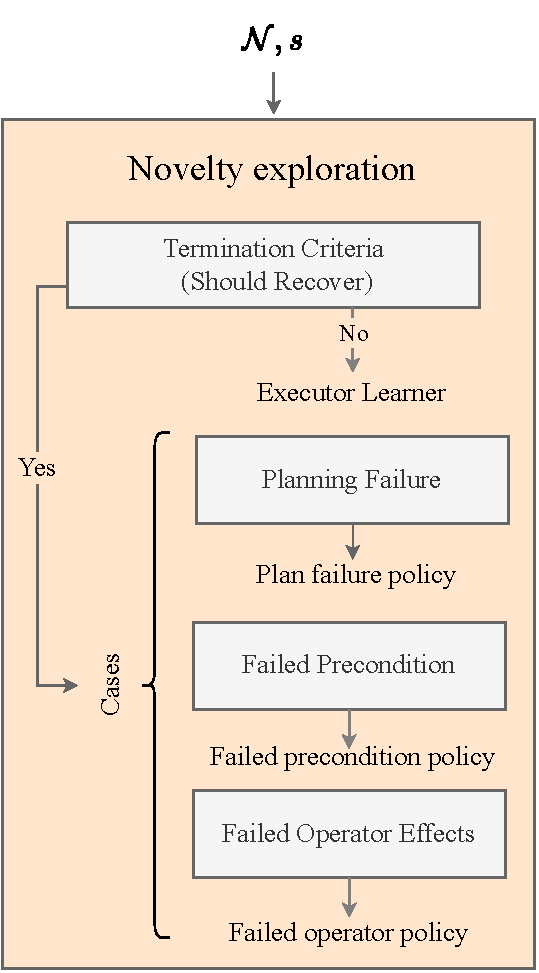
\includegraphics[width=0.30\linewidth]{figures/chapter5/novelty_explorer_component.pdf}\hspace{1.0cm}
    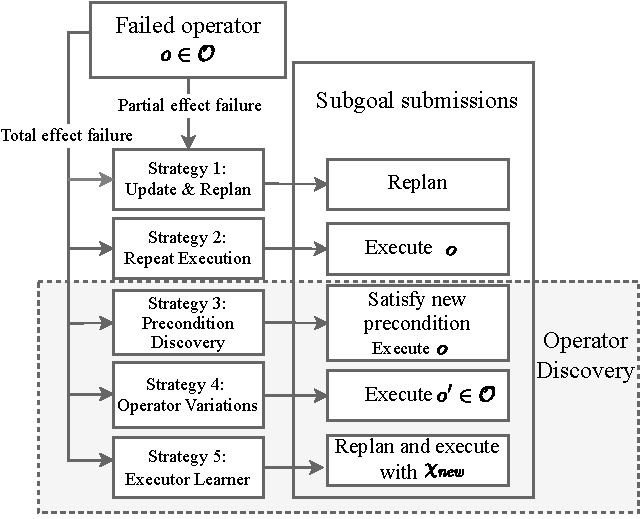
\includegraphics[width=0.55\linewidth]{figures/chapter5/failed_effect_policies.pdf}
    \caption{Diagrammatic representation of the agent's recovery policies. (Left) The recovery policies initiated under different failure conditions. (Right) The specific strategies of the failed-operator policy, applied when an operator's known effects are inconsistent with the observed state. Different recovery policies are initiated depending on how the novelty is encountered, and individual strategies may apply to multiple novelty types.}
    \label{fig:recovery_policies}
\end{figure}
}

\rev{\paragraph{Recovery from prohibitive novelty.} If the task planner fails to produce a plan, the exploration component follows a plan-failure policy driven by knowledge discovery. It generates and executes subgoals that prioritize operators exploring currently unobserved parts of the environment, updating the agent's prior knowledge where necessary. For instance, when the crafting table is missing from the state description, the agent explores ways to acquire one---opening the safe, visiting other rooms, or interacting with other actors---and replans once a solution is discovered. If knowledge discovery still fails to yield a plan, the executor learner is invoked to discover states from which a successful plan exists.}

\rev{\paragraph{Recovery from obstructive novelty.} Obstructive novelties surface as either precondition or effect failures, which are handled differently.}

\rev{\emph{Precondition failure.} An unmet precondition indicates that the agent's knowledge of the environment state is inaccurate (e.g.,\ a rival actor stole a resource after the plan was formed). The recovery strategy updates $\KB$ with the accurate state description obtained through the domain interface and prompts the planner to replan.}

When an operator's executor is executed but its effects are not observed in the resulting state, the architecture distinguishes between two cases:

\paragraph{Partial effect failure.} If a subset of the operator's expected effects are observed, the operator's description in $\KB$ is updated to reflect the observed effects, and the agent replans. This handles cases where an operator's behavior has changed but not disappeared entirely. \rev{Because the updated operator is re-exposed to the planner, this same mechanism automatically exploits beneficial novelties (when the revised effects enable a shorter plan) and ignores nuisance novelties (when the revised effects are irrelevant).}

\paragraph{Total effect failure.} If none of the operator's expected effects are observed, a cascading sequence of strategies is applied:
\begin{enumerate}[leftmargin=*]
    \item \emph{Update and replan}: The operator's effects are removed from $\KB$ and the agent attempts to find an alternative plan that avoids the failed operator.
    \item \emph{Repeated execution}: The operator is retried to account for stochastic or transient failures.
    \item \emph{Precondition discovery}: The agent hypothesizes that the operator requires an additional, previously unknown precondition. New preconditions are constructed from predicates encountered in the domain and tested by satisfying them before reattempting the operator. For instance, if \texttt{break(tree)} fails, the agent may hypothesize that \texttt{holding(axe)} is a missing precondition.
    \item \emph{Operator variations}: The agent tests known operators with similar parameters or on related objects, leveraging the type hierarchy in $\KB$ to discover operators with unexpected effects that may resolve the impasse.
    \item \emph{Executor learner (RAPid-Learn)}: If all symbolic strategies fail, the agent invokes the RAPid-Learn framework (\cref{sec:rapid_learn_method}) to learn a new executor through reinforcement learning with knowledge-guided exploration.
\end{enumerate}

\rev{Strategies 3 and 4 constitute the \emph{operator discovery} process described next, while strategy 5 is the knowledge-guided executor learner that forms the core of this chapter. The cascading design reflects a deliberate trade-off between computational cost and generality: symbolic strategies (steps 1--4) are fast but limited to novelties resolvable within the agent's existing representational vocabulary, whereas the executor learner (step 5) is more expensive but can discover recovery behaviors involving novel predicates, spatial relations, or action sequences absent from the original domain model---precisely the cases where symbolic reasoning is insufficient.}

\subsubsection{Operator Discovery}
\label{sec:operator_discovery}

\rev{When prohibitive or obstructive novelties are attributed to operator failure, the agent attempts to discover new operators that restore solvability. Two symbolic strategies are applied before the more expensive executor learner.}

\rev{\paragraph{Precondition discovery.} For a failed operator $\Operator$ with preconditions $\Pre_\Operator$, a new operator $\Operator'$ is constructed with the same effects and executor but an augmented precondition set. Candidate preconditions are drawn from all predicates encountered in $\Operators$ and added one at a time in a priority order (for example, by frequency in known operators or by domain-specific heuristics); the goal manager then attempts to satisfy the candidate and reattempt $\Operator'$. If the operator succeeds, the broken operator is replaced by $\Operator'$ in $\KB$. In the running example, when trees can no longer be broken without a tool, precondition discovery hypothesizes \texttt{holding(axe)} as a missing precondition of \texttt{break}, since holding a tool is already a precondition for breaking other resources.}

\rev{\paragraph{Operator variations.} If precondition discovery fails, the agent searches for known operators with unexpected effects, guided by the type hierarchy in two phases. First, it attempts other operators that accept the same parameters as the failed one (e.g.,\ operators that take a tree, when \texttt{break(tree)} fails). Second, it prioritizes operators acting on different parameters of the same type (e.g.,\ retrying the operator on an oak tree when it failed on a birch tree). If any variation produces unexpected effects, a new operator is added to $\KB$ and the agent replans.}

\rev{\paragraph{Knowledge-guided executor learner.} Because the search spaces for precondition discovery and operator variations grow exponentially, they cannot be searched exhaustively. After bounded effort in these directions, the agent invokes a reinforcement-learning-based executor learner that creates a new executor for the failed operator, using a reward function encoding the operator's desired effects and biasing exploration toward states and actions related to the detected novelty. This learner is the RAPid-Learn framework, which we describe in full detail in \cref{sec:rapid_learn_method} after formalizing the executor discovery problem it solves in \cref{sec:executor_discovery}.}
